\section{Reticoli}
\subsection{Reticolo}
\bottom{
    Sia \((s, \rho)\) un insieme ordinato, con \(\rho \in OL(s)\). Allora:
    \((s, \rho)\) è un reticolo \(:\iff\) $$\forall x,y \in s$$
    $$ \exists z, w \in s$$ $$ z = INF_{(s, \rho)}(\{x, y\}) \land w = SUP_{(s, \rho)}(\{x, y\})$$

    Cioè l'insieme di ogni coppia di elementi di \(s\) è dotato di estremo superiore ed inferiore in \(s\).
}

\subsection{Operazioni in un Reticolo}
\bottom{
        Dato un reticolo $(s, \rho)$, possiamo definire, \(\forall x, y \in s\):
    \begin{align*}
        &\text{Intersezione reticolare}\\
        &&&\wedge: (x, y) \in s \times s \mapsto INF_{(s, \rho)}(\{x, y\}) \in s\\
        &\text{Unione Reticolare}\\
        &&&\vee: (x, y) \in s \times s \mapsto SUP_{(s, \rho)}(\{x, y\}) \in s
    \end{align*}
    Cioè due operazioni binarie ed interne.
}

\subsection{Notazione di Reticolo come Struttura}
\bottom{
    Dato un reticolo \((s, \rho)\), dato che possiamo definire in esso due operazioni binarie interne \(\vee\) e \(\wedge\), allora possiamo notarlo come una struttura: \((s, \wedge, \vee)\)
}

\subsection{Reticolo Limitato}
\bottom{
    Un reticolo \((s, \rho)\) si dice limitato se è dotato di minimo e massimo.
}

\subsection{Reticolo Completo}
\bottom{
    Un reticolo \((s, \rho)\) si dice completo se ogni sua parte non vuota è dotata di estremi superiore ed inferiore.
    Ogni reticolo completo è anche un reticolo limitato.
}

\subsection{Estremi di Coppie di Elementi Confrontabili di un Reticolo}
\bottom{
    Dato un reticolo \((s, \rho)\) e due elementi \(x, y \in s\). Siano essi confrontabili, ad esempio \(x \rho y\). Allora:

    $$INF_{(s,\rho)}(\{x, y\}) = (x \wedge y) = x$$
    $$SUP_{(s,\rho)}(\{x, y\}) = (x \vee y) = y$$
}
\bottomp{
    \(x \rho x\) per riflessività di \(\rho\) (che, essendo \(s\) un reticolo, deve necessariamente essere d'ordine largo). Per ipotesi, \(x \rho y\). Dunque \(x\) è minimo di \(\{x, y\}\), e quindi è anche estremo inferiore.
    Analgoamente si dimostra per l'estremo superiore.
}

\subsection{Enunciato Duale sui Reticoli}
\bottom{
    Sia \((s, \rho)\) un reticolo, e \((s, \overline\rho)\) il suo reticolo duale. Se \(e\) è un enunciato sui reticoli, dico enunciato duale \(\overline e\) l'enunciato ottenuto:

    - Rimpiazzando ogni \(\rho\) in \(e\) con \(\overline \rho\) (e viceversa)

    - Rimpiazzando ogni \(\wedge\) in \(e\) con \(\vee\) (e viceversa)
}

\subsection{Principio di Dualità Per i Reticoli}
\bottom{
    Se \(e\) è una formula valida per ogni reticolo, allora anche la sua duale \(\overline e\) lo è.
}
\bottomp{
    \(e\) è valida per ogni reticolo \((s, \rho)\), ma quindi è valida anche per il suo duale \((s, \overline\rho)\). Ma nel reticolo duale, gli estremi inferiori sono estremi superiori e viceversa. Dunque, \(e\) riferito a \((s, \overline\rho)\) è esattamente \(\overline e\) riferito a \((s, \rho)\).
}

\subsection{In un Reticolo ogni Minimale è Minimo e ogni Massimale è Massimo}
\bottomp{
    Dimostriamo per i minimali, per dualità vale anche per i massimali.

    Sia \((s, \rho)\) un reticolo e sia \(m \in s\) minimale. Sia \(x \in s\) un elemento generico del reticolo. Allora si ha che $$(m \wedge x)\ \rho\ m$$ per la definizione di estremo inferiore. Ma quindi \(m \wedge x\) ed \(m\) sono confrontabili, e dunque per la definizione di minimale, $$m\ \rho\ (m \wedge x)$$ Dunque per asimmetria \(m \wedge x = m\), per ogni \(x \in s\), e allora \(m\) è mimimo di \(s\).
}

\subsection{In un Reticolo I Minoranti (Maggioranti) dell'Unione sono l'Intersezione dei Minoranti (Maggioranti) di Parti Finite}
\bottom{
    Sia \((s, \rho)\) un reticolo e siano \(a, b \in P(s)\) finiti. Allora:
$$MINOR_{(s, \rho)}(a \cup b) = MINOR_{(s, \rho)}(a) \cap MINOR_{(s, \rho)}(b)$$
Per dualità vale l'analogo per i maggioranti.
}
\bottomp{
    \begin{align*}
        x \in MINOR_{(s, \rho)}(a \cup b) &\iff \forall y \in a \cup b\ (x \rho y)  \\
        &\iff \forall y\ (y \in a \lor y \in b \implies x \rho y)  \\
        &\iff \forall y\ (y \in a \implies x \rho y) \land \forall y\ (y \in b \implies x \rho y) \\
        &\iff x \in MINOR_{(s, \rho)}(a) \land x \in MINOR_{(s, \rho)}(b) \\
        &\iff x \in MINOR_{(s, \rho)}(a) \cap MINOR_{(s, \rho)}(b) 
    \end{align*}
}

\subsection{I Minoranti (Maggioranti) di un Insieme Ordinato sono i Minoranti (Maggioranti) dell'Estremo Inferiore (Superiore)}
\bottom{
    Sia \((s, \rho)\) un insieme ordinato e sia \(a \subseteq s\). Se esiste \(m = INF_{(s,\rho)}(a)\), allora:

    $$MINOR_{(s,\rho)}(a) = MINOR_{(s,\rho)}(\{m\})$$
}
\bottomp{
    Questo deriva semplicemente dal fatto che l'estremo inferiore è il massimo dei minoranti.
}

\subsection{Ogni Parte Finita di un Reticolo è dotata di Estremo Inferiore e Superiore}
\bottom{
    Sia \((s, \rho)\) un reticolo. Ogni sua parte finita è dotata di estremo inferiore e superiore.
}
\bottomp{
    Siano \(a, b \in P(s)\) due insiemi finiti. Allora:
    1) Per "I Minoranti (Maggioranti) dell'Unione sono l'Intersezione dei Minoranti (Maggioranti) degli Insiemi Finiti" e per "I Minoranti (Maggioranti) di un Insieme sono i Minoranti (Maggioranti) dell'Estremo Inferiore (Superiore)" abbiamo che:

    Siano $$m_1 = INF_{(s, \rho)}(a)$$
    $$ m_2 = INF_{(s, \rho)}(b)$$
    \begin{align*}
        &MINOR_{(s, \rho)}(a \cup b) =\\
        & MINOR_{(s, \rho)}(a) \cap MINOR_{(s, \rho)}(b) =\\
        & MINOR_{(s, \rho)}(\{m_1\}) \cap MINOR_{(s, \rho)}(\{m_2\}) =\\
        &MINOR_{(s, \rho)}(\{m_1, m_2\})
    \end{align*}

    2) Dimostriamo per induzione su \(n = |t|\) dove \(t\) è una parte finita di \(s\).
    Caso base: \(n = 1\). Allora \(t\) è un singleton, ed il suo unico elemento è (per riflessività) sia estremo superiore che estremo inferiore.
    Assumendo adesso che la tesi induttiva sia valida per ogni \(1 \leq k < n\), dimostriamo per \(n\).
    Sia \(x \in t\). Allora $$t = (t - \{x\}) \cup \{x\}$$ cioè l'unione di un insieme di ordine \(n-1\) e di uno di ordine \(1\). Per ipotesi induttiva, allora essi sono dotati di estremi inferiori, con $$m = INF_{(s, \rho)}(t - \{x\})$$
    $$ x = INF_{(s, \rho)}(\{x\})$$
    Allora, per la (1):
    $$
    MINOR(t) = MINOR((t - \{x\}) \cup x) = MINOR(\{m, x\}).
    $$

    Dato che siamo in un reticolo, la coppia \(\{m, x\}\) ha sicuramente estremo inferiore, cioè $$max(MINOR(\{m, x\})) = max(MINOR(t))$$ da cui la tesi.

    Per dualità, lo stesso vale per l'estremo superiore.
}

\subsection{Commutatività di \(\wedge\) e \(\vee\)}
\bottom{
    Sia \((s, \wedge, \vee)\) un reticolo. Allora:
    $$\forall x, y \in s\ ((x \wedge y = y \wedge x) \land (x \vee y = y \vee x))$$
}
\bottomp{
    $$x \wedge y = INF_{(s, \rho)}(\{x, y\}) = INF_{(s, \rho)}(\{y, x\}) = y \wedge x$$
    $$x \vee y = SUP_{(s, \rho)}(\{x, y\}) = SUP_{(s, \rho)}(\{y, x\}) = y \vee x$$
}

\subsection{Associatività di \(\wedge\) e \(\vee\)}
\bottom{Sia \((s, \wedge, \vee)\) un reticolo. Allora \(\wedge, \vee\) sono associative.}
\bottomp{
    Dimostriamo per \(\vee\), la dimostrazione per \(\wedge\) è analoga per dualità.

    Siano \(x, y, z \in s\). Per definizione abbiamo che:
    \begin{itemize}
        \item \(x \rho [x \vee (y \vee z)]\)
        \item \((y \vee z) \rho [x \vee (y \vee z)]\)
        \item  \(y \rho (y \vee z)\)
        \item \(z \rho (y \vee z)\)
    \end{itemize}

    Allora per transitività:
    $$y \rho [x \vee (y \vee z)]$$

    $$z \rho [x \vee (y \vee z)]$$

    E dunque:
    $$(x \vee y) \rho [x \vee (y \vee z)]$$

    Ed infine:
    $$[(x \vee y) \vee z] \rho [x \vee (y \vee z)]$$

    Lo stesso procedimento si può fare nel senso opposto per dimostrare che $$[x \vee (y \vee z)] \rho [(x \vee y) \vee z]$$
    Dunque, per asimmetria:
    $$[(x \vee y) \vee z] = [x \vee (z \vee y)]$$
}

\subsection{Proprietà di Assorbimento di un Reticolo}
\bottom{
    $$\forall x, y \in s\ ((x \vee (x \wedge y) = x) \land (x \wedge (x \vee y) = x))$$
}

\subsection{Proprietà di Idempotenza/Iteratività di \(\wedge\) e \(\vee\)}
\bottom{
    In un reticolo \((s, \rho)\) $$\forall x  \in s\ (x = x \vee x = x \wedge x )$$
}
\bottomp{
    Dimostriamo per \(\wedge\), analogo per \(\vee\).
    Dalle proprietà di assorbimento, segue che:
    $$\forall y \in s\ (x \wedge (x \vee y) = x)$$
    Dato che \(x \wedge x \in s\), allora, ponendo \(y = x \wedge x\) e applicando ancora una volta l'assorbimento:
    $$x = x \wedge (x \vee (x \wedge x)) = x \wedge x $$
}

\subsection{Corrispondenza Biunivoca fra Reticoli e Strutture}
\bottom{
    Sia \(s\) un insieme non vuoto e sia \(r\) l'insieme delle relazioni d'ordine largo \(\rho\) per cui \(s\) è un reticolo.
    Sia \(b\) l'insieme delle coppie di operazioni binarie interne \((\alpha, \beta)\) tali che entrambe siano commutative, associative, e valga la legge di assorbimento in \((s, \alpha, \beta)\)
    Allora l'applicazione $$f: \rho \in r \mapsto (\wedge_\rho, \vee_\rho) \in b \text{ è biettiva}$$ Cioè, da ogni reticolo si possono definire $\wedge$ e $\vee$, e ogni coppia di operazioni associative, commutative, idempotenti, e per cui vale l'assorbimento sono $\wedge$ e $\vee$ di un qualche reticolo.
}
\bottomp{
    Per dimostrare che \(f\) è biettiva, vogliamo trovare la sua inversa. Siano \((\wedge, \vee) \in b\) e definiamo \(\rho\) tale che $$\forall x, y \in s\ (x \rho y \iff x = x \wedge y)$$
    Nota che da questo segue che \(x \vee y = (x \wedge y) \vee y = y\) per assorbimento.

    1) \(\rho\) così definita è di ordine largo? Per idempotenza, $$x \wedge x = x \implies x \rho x$$ quindi vale la riflessività. Se $$(x = x \wedge y) \land (y = y \wedge x)$$ dato che $\wedge$ è ipotizzata commutativa, \(x = y\) e quindi vale l'asimmetria.
    Se \(x \rho y \land y \rho z\), allora $$(x = x \wedge y) \land (y = y \wedge z)$$ Quindi, per associatività: $$x = x \wedge (y \wedge z) = (x \wedge y) \wedge z = x \wedge z \implies x \rho z$$ quindi vale la transitività.\\
    \(\rho\) è effettivamente una relazione d'ordine largo.

    2) Vogliamo far vedere che $$INF_{(s, \rho)}(\{x, y\}) = x \wedge y$$ e che $$SUP_{(s, \rho)}(\{x, y\}) = x \vee y$$ per ogni \(x, y \in s\).
    Per assorbimento $(x \wedge y) \vee x = x$ quindi per definizione abbiamo che $(x \wedge y) \rho x$.\\
    Analogamente $(x \wedge y) \rho y$.\\
    Quindi $$x \wedge y \in MINOR_{(s, \rho)}(\{x, y)\}$$ Vogliamo far vedere che \(x \wedge y\) è il massimo dell'insieme. Sia dunque \(z\) un generico minorante. Allora si ha:
    $$z\rho y \land z \rho x \implies (z = z \wedge y) \land (z = z \wedge x)$$
    E quindi:
    \(z = z \wedge x = (z \wedge y) \wedge x = z \wedge (x \wedge y) \implies z \rho (x \wedge y)\) da cui la tesi che \(x \wedge y\) è estremo inferiore.
    Lo stesso procedimento vale, analogamente, per gli estremi superiori.

    Si osserva semplicemente che la funzione \((\wedge, \vee) \in b \mapsto \rho \in r\) è l'inversa di \(f\), da cui la tesi.
}

\subsection{Isomorfismo fra Reticoli}
\bottom{
    Siano \((s, \wedge, \vee), (s', \wedge', \vee')\) due reticoli. Allora \(f: s \to s'\) si dice isomorfismo fra i due reticoli se:

    1) \(f\) è biettiva

    2) $\forall x, y \in s\ ((f(x \wedge y) = f(x) \wedge' f(y)) \land (f(x \vee y) = f(x) \vee' f(y)))$
}

\subsection{Equivalenza fra Isomorfismo di Reticoli e Isomorfismo di Insiemi Ordinati}
\bottom{
    Siano \((s, \wedge, \vee), (s', \wedge', \vee')\) due reticoli e sia \(f: s \to s'\) una funzione biettiva fra i due. Allora:
    \(f\) isomorfismo fra i reticoli \(\iff\) \(f\) è un isomorfismo di insiemi ordinati fra \((s, \rho_{(\wedge, \vee)})\) e \((s', \rho_{(\wedge', \vee')})\)
}
\bottomp{
    Dimostrazione \(\Leftarrow)\):

    Siano \((s, \rho), (s', \rho')\) due reticoli e sia \(f\) un isomorfismo di insiemi ordinati fra essi. I reticoli possono essere espressi come strutture \((s, \wedge_\rho, \vee_\rho), (s', \wedge_{\rho'}, \vee_{\rho'})\)

    Si ha che: $$\forall x, y \in s$$
    $$(x \wedge_\rho y) \rho x$$
    $$(x \wedge_\rho y) \rho y$$
    Applicando l'isomorfismo: $$f(x \wedge_\rho y) \rho' f(x)$$
    $$f(x \wedge_\rho y) \rho' f(y)$$
    Quindi $$f(x \wedge_\rho y) \in MINOR_{(s', \rho')}(\{f(x), f(y)\})$$
    Sia \(z \in MINOR_{(s', \rho')}(\{f(x), f(y)\})\).

    Si ha che $$z \rho' f(x)$$
    $$z \rho' f(y)$$
    Essendo \(f\) suriettiva, $\exists w \in s\ (f(w) = z)$.
    Allora, applicando l'isomorfismo in senso inverso $w\rho x \land w \rho y$. Quindi \(w\) è minorante di \(\{x, y\}\).
    Allora si ha che:
    $$w \rho (x \wedge_\rho y) \implies f(w) \rho' f(x \wedge_\rho y) \implies z \rho' f(x \wedge_\rho y)$$
    E quindi \(f(x \wedge_\rho y)\) è estremo inferiore di \(\{f(x), f(y)\}\), cioè:
    $$f(x \wedge_\rho y) = f(x) \wedge_{\rho'} f(y)$$ che è la tesi.
    Analogamente si dimostra per \(\vee\).

    Dimostrazione \(\Rightarrow\):
    Sia \(f\) isomorfismo fra \((s, \wedge, \vee), (s', \wedge', \vee')\) e siano \(\rho, \rho'\) le relazioni d'ordine associate.
    Prendiamo \(x, y \in s: x \rho y\). Per definizione \(x = x \wedge y\) e quindi $$f(x) = f(x \wedge y) = f(x) \wedge' f(y) \iff f(x) \rho' f(y)$$
    Questo vale in entrambi i versi (in quanto è una catena di uguaglianze seguita da un'equivalenza materiale) e quindi abbiamo la tesi.
}

\subsection{Sottoreticolo}
\bottom{
    Sia \((s, \wedge, \vee)\) un reticolo e sia \(t \in P(s) - \{\emptyset\}\).\\
    Se \(t\) è parte chiusa rispetto \(\wedge, \vee\).\\
    $(t,\wedge,\vee)$ si dice sottoreticolo di \((s, \wedge, \vee)\).
}

\subsection{Intervallo e Intervallo Chiuso}
\bottom{
    Sia \((s, \rho)\) un insieme ordinato, con \(\rho \in OL(s)\).

    \(i \subseteq s \text{ intervallo } :\iff\)
    $$ \forall x, y \in i$$
    $$ \forall z \in s$$
    $$(x\rho z \land z \rho y \implies z \in i)$$

    In particolare, se \(i\) è limitato, si dice intervallo chiuso.
}

\subsection{Ogni Intervallo Chiuso di un Reticolo è un Sottoreticolo}
\bottom{
    Se \((s, \rho)\) è un reticolo, ogni suo intervallo chiuso è un sottoreticolo.
}
\bottomp{
    Sia \(i \in s\) un sottointervallo. Allora, dati \(x, y \in i\), esiste estremo inferiore \(x \wedge y \in s\). $$min(i) \rho x \land min(i) \rho y \implies min(i) \rho (x \wedge y) \rho x \implies x \wedge y \in i$$
    Procedimento analogo si effettua per l'estremo superiore.
}

\subsection{Massimo e Minimo sono Elementi Neutri di un Reticolo (e Viceversa)}
\bottom{
    Sia \((s, \rho)\) un reticolo. Siano \(m, M \in s\). Allora:

    \(m \text{ minimo di } s \iff m \text{ neutro di } \vee_\rho\)

    \(M \text{ massimo di } s \iff M \text{ neutro di } \wedge_\rho\)
}
\bottomp{
    \(\Rightarrow)\) Sia \(x \in s\). Allora \(x \rho M \land x \rho x\). Dunque \(x = min(\{x, M\}) = x \wedge_\rho M\). Dunque \(M\) è neutro.

    \(\Leftarrow)\) \(\forall x \in s\ (M\wedge_\rho x =x) \implies \forall x \in s\ (x \rho M)\).

    Analogamente si dimostra per il minimo.
}

\subsection{Reticolo Complementato}
\bottom{
    Un reticolo limitato \((s, \rho)\) si dice complementato se:
    $$\forall x \in s,\ \exists y \in s$$
    $$ (x \wedge y = min(s) \land x \vee y = max(s))$$

    E si dice che \(x\) è complementato e che \(y\) è il suo complemento.
}


\subsection{Elementi Confrontabili e Complementati di un Reticolo sono il Minimo e il Massimo}
\bottom{
    Sia \((s, \rho)\) un reticolo complementato. Allora:
    Due elementi \(x, y \in s\) sono confrontabili e complementati \(\iff\) uno è il minimo e l'altro è il massimo.
}
\bottomp{
    Se i due elementi sono confrontabili, allora essi sono rispettivamente il minimo e massimo della loro coppia, e sono quindi anche estremo inferiore e superiore. Ma essendo i due elementi complementari, per ipotesi, allora si ha che il loro estremo inferiore è il minimo ed il loro estremo superiore è il massimo. Perciò essi coincidono.
}

\subsection{Reticolo Distributivo}
\bottom{
    Un reticolo \((s, \wedge, \vee)\) si dice distributivo se valgono entrambe le Leggi Distributive:
    $$\forall a, b, c \in s\ (a \wedge (b \vee c) = (a \wedge b) \vee (a \wedge c))$$
    $$\forall a, b, c \in s\ (a \vee (b \wedge c) = (a \vee b) \wedge (a \vee c))$$
    Si dimostra che se in un reticolo vale una legge di distributività, allora vale anche l'altra. Dunque, per essere un reticolo distributivo, basta che valga una delle due leggi dato che l'altra segue.
}

\subsection{Unicità dei Complementi di Reticoli Distributivi}
\bottom{
    Sia \((s, \rho)\) un reticolo distributivo limitato. Allora ogni complemento è unico.
}
\bottomp{
    Sia \(x \in s\) e siano \(y, z \in s\) suoi complementi. Allora:
    $$y = y \wedge max(s) = y \wedge (x \vee z) = (y \wedge x) \vee (y \wedge z) = min(s) \vee (y \wedge z) = y \wedge z$$

    E cioè \(y \rho z\). Effettuando il procedimento analogamente per \(z\), otteniamo \(z \rho y\). Dunque \(y = z\) per asimmetria.
}

\subsection{Criterio di Distributività di Birkhoff}
\bottom{
    Un redicolo è distributivo \(\iff\) non contiene sottoreticoli isomorfi al Reticolo Trirettangolo o al Reticolo Pentagonale.

    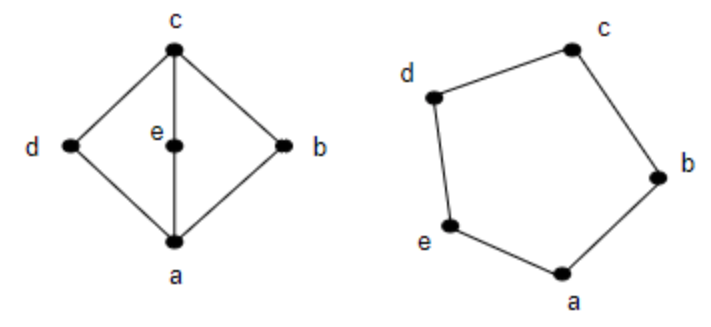
\includegraphics[scale=0.2]{img/Birkhoff.png}

    Osservazioni:

    Un reticolo totalmente ordinato è sempre distributivo.

    Tutti i reticoli di ordine $n<5$ sono distributivi.
}